\chapter{Methodology}
\label{chap:methodology}

% This study consists of a design of the proposed method, an implementation of this design, and several test to assess this implementation. 
This chapter present the design of the proposed method. 
It first sums up and clarifies all requirements of the method, proceeded by presenting and overview, followed up by the various aspects to the design of the method. 
It finishes by elaborating on the assessments used to test the environment. 

\section{Definitions}

Throughout this and subsequent chapters, the following terms and phrases will be used.
% No claims are made that these exact definitions are canonical, they simply seemed appropriate for the situation.

\textbf{Pipeline / Script}: A program 'written' within a VPL is referred to as a 'script' or a 'pipeline'.

\textbf{VPL as Programming Language or Application}: An ambiguity exist of calling a VPL an application or a programming language. 
Arguments can be made for both. 
This study would describe its VPL as an application, which happens to possess a composable \ac{GUI}, and not a programming language.
Nevertheless, depending on context, the VPL will be referred to as both.

\textbf{Plugin vs Library}: A plugin represents additional, optional functionalities for a certain application.
A library represents additional functionalities to be used within a programming language. 
Due to aforementioned ambiguity of a VPL, 'additional functionalities' for a VPL could be called both. 
To make matters worse, the upcoming plugin system will blur the lines between library and plugin. 
To offer some clarification, the term 'plugin' will be used when referring to the 'functionalities' from a point of view of the VPL.
The term 'library' will be reserved for referring to a software library itself. 

\textbf{Node}: a component or 'block' within a VPL pipeline. It is analogous to a function in a normal language.

\textbf{Boilerplate}: An informal term to refer to code which is not part of the core logic of an application. It is in a sense irrelevant code, but still required in order to use a certain system or feature. 

\textbf{Binding}: Bindings refer to the code a maintainer of a library may add to allow it to be used in another language. For example, a C++ library can have python bindings. 
Bindings may sometimes be regarded as boilerplate.

\textbf{Headless}: Headless execution of a program means that it is run without using its normal \ac{GUI}. 
Often, this means a \ac{CLI} is used instead.

\section{Requirements}
\label{sec:method:require}

Three supporting research questions ask to clarify requirements for the design of the methodology. 
These questions can now be partially answered based on the literature presented at \refchap{chap:background} and \refchap{chap:related}, and based on insights granted by these works.
The answers to these questions form the core requirements of the proposed method, and steer its features and design considerations.

\begin{itemize}[ ]
  \item \emph{What GUI features are required to facilitate this method? (and to what extent does the
  web platform aid or hurt these features?)}  
\end{itemize}

Two layers of \ac{GUI} features are required:

\textbf{Framework application}: Firstly, a base web application is required to host the visual programming language.
This needs to provide a \ac{GUI} for all basic application features, like saving, loading, undoing and redoing.

\textbf{The VPL}: Secondly, UI elements are required to form the interactive elements of the visual program itself. 
This forms a layer independent from the framework application, and will require a custom set of \ac{GUI} features. 
That is to say, a text field within the framework is not the same as a text field within the visual program.
Existing VPLs differ in their level of support of certain '\ac{GUI} nodes'.
This study has established that extensive support is required, for the sake of visualizing geodata, and parametrization of \ac{GIS} operators.

\begin{itemize}[ ]
  \item \emph{To what extent does this method intent to address the discrepancies between software
applications and libraries, as described by Elliott (2007) (Does it succeed in doing so?)}
\end{itemize}

All three discrepancies described by the introduction \\ are addressed by incorporating the following aspects: \\

\textbf{Generic GUI}: The VPL must serve as a generic \ac{GUI} to serve practically any \ac{GIS} library. 
As such, it requires a wide range of buttons, sliders, text fields, and other inputs.

\textbf{Composable applications}: In order to make web applications themselves more composable, the \ac{GUI} of the VPL itself should incorporate other web applications, via for example a \m{<iframe>} or popup.

\textbf{Direct utilization}: To allow direct utilization of a library, the solution must be distributed as a static web application. 
To make sure library capabilities do not get lost when used in an application, the VPL must be able to accept a wide range of libraries as plugins, with as little bindings or glue code as possible.


\begin{itemize}[ ]
  \item \emph{What measures are taken to make this VPL scalable to large geo-datasets? (and how
  effective are these measures?)}
\end{itemize}

Three measures will be taken to offer scalability in principle: 

\textbf{Portability}: A Backend execution of a VPL pipeline must be predictable. 
As such, GIS libraries run on the frontend by the VPL must behave exactly the same as if they were run on a backend. 

\textbf{Zero-cost abstraction}: A pipeline created with the VPL should be able to run headless, to ensure a scalable backend can use such a pipeline.

\textbf{Locality}: The VPL should be designed as a Dataflow VPL, which shares characteristics with functional programming. This leads to source code which can be reasoned about in a local manner, instead of a global one. This allows for parallelization when scaled in a backend environment.

\section{Overview}

\graphicspath{{../../assets/images/1/}}

\begin{figure}
  \centering
  \begin{subfigure}[b]{0.80\linewidth}
    \centering
    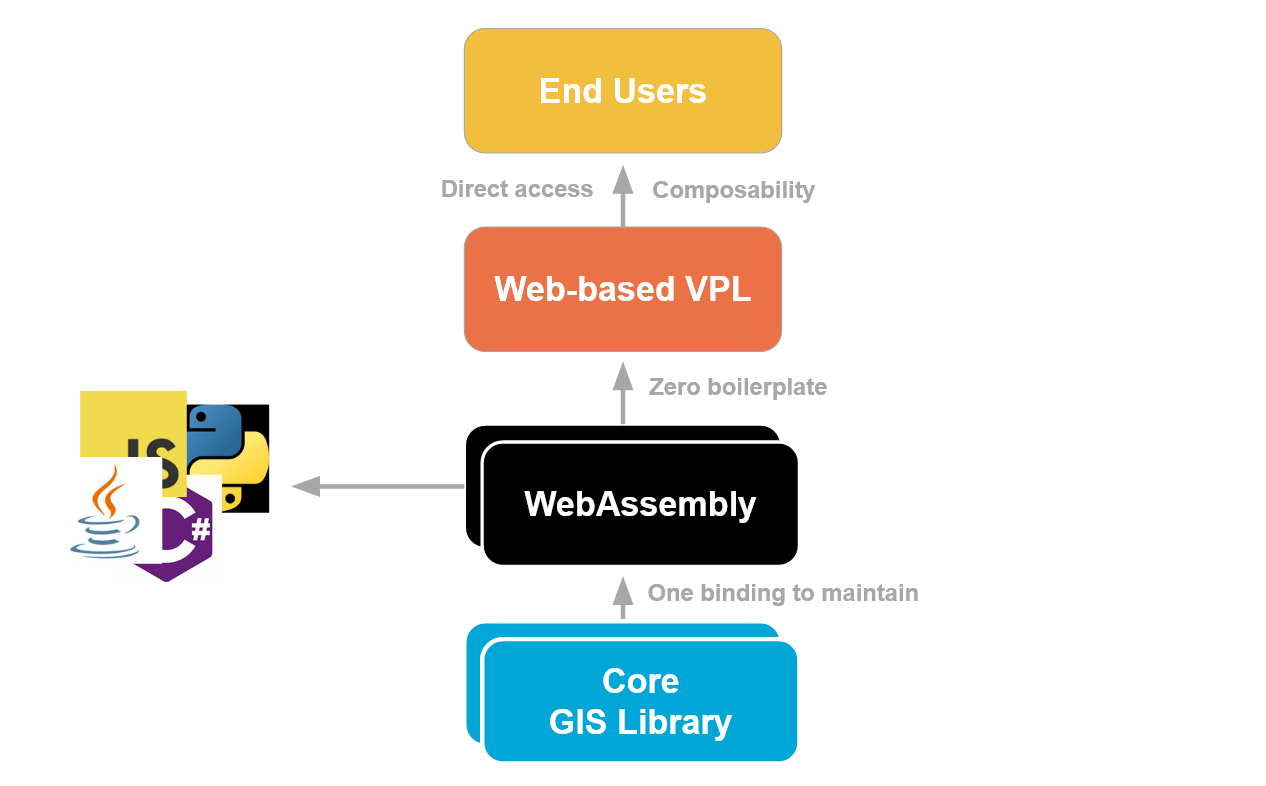
\includegraphics[width=\linewidth]{proposal.png}
  \end{subfigure}%
  \caption{The proposed methodology}
  \label{fig:proposal}
\end{figure}

The design of this method is as visualized by \reffig{fig:proposal}: 
A Prototype VPL is used to host the functionalities of \ac{GIS} libraries from within an application, and in a composable manner. Additionally, it is used to connect these libraries to various \ac{GUI} features. 
The format of web application is used to allow this prototype to be directly accessible to end users without installation or configuration. 
% Geodata used within the application is also exclusively statically hosted geodata, or user-submitted data. 
This prototype is statically hosted, to minimize operational costs.
\ac{GIS} libraries are loaded within this platform by first compiling them into WebAssembly, and then loading this binary as a plugin directly. 
This method is dubbed a 'no-boilerplate' method, and explores how libraries can be used with as little in-between layers as possible.
WebAssembly is also used to that libraries written in native languages can be used without resorting to active backend web services. 
Finally, as this prototype is intended for \ac{GIS} usage, both scalability to handle sizable datasets, and rich \ac{GUI} support (3D viewers, file inputs, sliders), are primary design considerations and assessment criteria. 
% prototypes aspires to qualify as a \ac{VPL}

\section{Framework Application}

To serve the requirements of a \textbf{Framework application} and \textbf{direct utilization}, a framework web application will be required. 
A UI library akin to imgui \citep*{cornut_dear_2022} or egui \citep*{ernerfeldt_egui_2022} would be optimal in providing such an environment. 
However, due to the absence of such a desktop application-like framework in the JavaScript ecosystem, a custom implementation will be needed. 
Using HTML5 features like Web Components, custom components such as multiple windows, dropdown menu's, side menu's etc. can be created without resorting to JavaScript frameworks.

\section{Web VPL} 
\label{sec:method:base-vpl}

Secondly, a web-based VPL is required as a host for all subsequent steps of the methodology. 
This VPL must serve the requirements of \textbf{The VPL}, a \textbf{Generic GUI}, \textbf{Composable applications} and \textbf{Locality}.

A novel, custom VPL is needed to fit all requirements. 
A dataflow VPL must be designed for web usage, which offers a range of \ac{GUI} nodes to serve as a generic GUI, and to allow applications to be composable. 

While the initial plan was to re-use an existing web VPL, the related works review of \refchap{chap:related} showcased that no exiting browser-based geocomputation VPL would be an appropriate fit.
The Mobius Modeller \citep{janssen_mobius_2021} came closest, but offered no dataflow VPL, no GUI components, and no plugin support. 
Additionally, the sizable nature of the mobius modeller project made aligning its goals with the goals of this study challenging. 
Building a custom implementation would also allow more degrees of freedom.

The following approach was deemed as the most fitting method for implementing this VPL. 
First, the components of a dataflow-VPL handling geometry have to be made clear.
Secondly, in order to know what tools may be used to implement this VPl, a small analysis of "widely supported browser features" is made. 
Then, with both these constraints known, a design for a web VPL can be layed out, which can be subsequently implemented. 

\subsection{Components}

The components of a dataflow-VPL implementation can be subdivided in components of a dataflow VPl in general, and a VPL for geo-computation specifically.
Based on the literature study of \refsec{sec:background-vpl}, any dataflow-VPL must at least contain the following aspects: 
\begin{enumerate}[-]
  \item a base 'programming language model'
  \subitem A representation of the 'variables' and 'functions' of the language
  \subitem With all computations being pure functions
  \subitem With all variables being immutable
  \item a 'graph-like' visualization of this data model
  \item an interface to create and edit this graph 
  \item a way to provide input data 
  \item a way to execute the language
  \item a way to display or save output data
\end{enumerate}
The implementation of these aspects would result in a 'baseline', general purpose, dataflow VPL. 
To specialize this implementation further, A visual programming language handling geometry should have:
\begin{enumerate}[-]
  \item Type safety 
  \item A way to load or to create geometry data 
  \item A way to export geometry data
  \item A method to preview geometry data in 3D
  \item A standard set of geometric types and operations
\end{enumerate}
These requirements need further explanation.
First, regarding type safety.
In this context, type safety refers to: 
The input and output of a function should have a type stated, and users should be notified of incorrect usage of types, or 'invalid connections'.
Geometry VPLs in particular need this, as many data representations of geometry are required to be precise about their data usage.
A VPL used to construct geometry should reflect this.
Additionally, when these types are clear and clearly communicated, users must have ways to provide these types as inputs or outputs. 
This will require specialized parsers to become part of the VPL, such as an obj and geojson reader and writers. 

Regarding visualization, A hallmark of VPLs is the ability to inspect the data of in-between steps, so this must be provided for.
This is also a good fit, since the immutable nature of dataflow VPL variables make these variables ideal for caching. 

Finally, a geometry VPL should contain a set of 'internal', basic types and operations.
All aforementioned features are difficult to implement without defining some set of internally recognized data types. 
Basic operations are needed in particular to transform between the types.

\subsection{Widely supported browser features}

\begin{figure}
  \centering
  \graphicspath{ {../../assets/plots/browser-usage/} }
  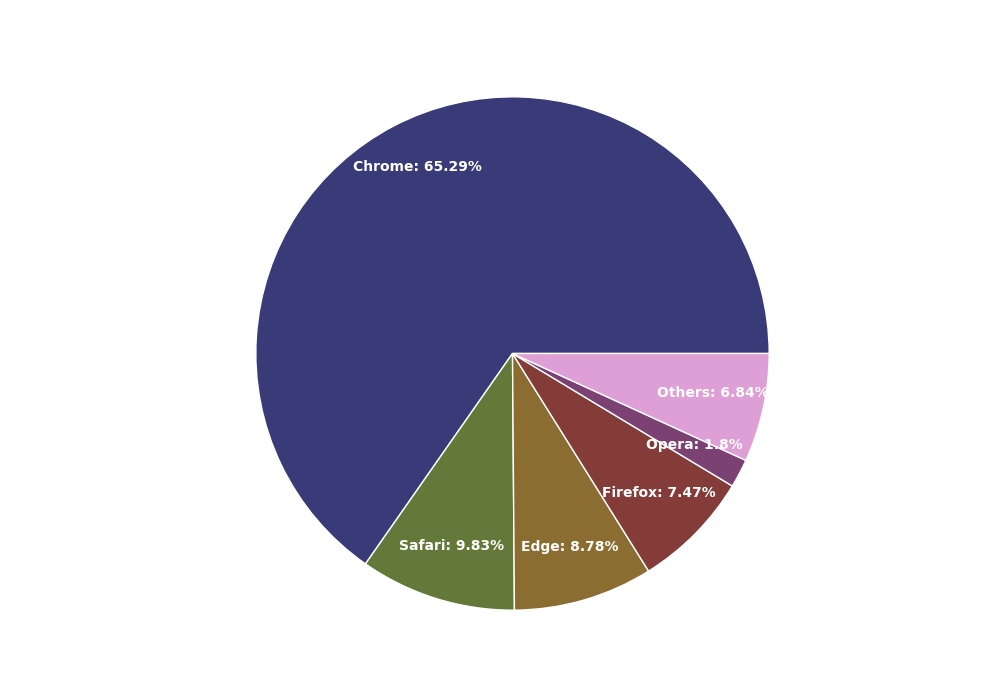
\includegraphics[width=0.7\linewidth]{plot.png}
  \caption[Browser usage]{Fall 2021 desktop browser usage statistics. Data averaged over (\citep{dashiki_simple_2020,w3counter_global_2020,the_netmarketshare_team_browser_2020,statcounter_global_stats_browser_2020})}
  \label{fig:browser-usage}
\end{figure}

This study defines "widely supported browser features" as the set of default features implemented by the browser engines of 'major browsers'. 
Based on the desktop browser market shares of \reffig{fig:browser-usage}, the chromium based browsers (Chrome, Edge, Opera) have the majority. 
This is followed up by Firefox, based on the Gecko engine, and Safari, based on webkit. 
By supporting these three engines, the vast majority of end-users can be served.

The set of features common in these three browser engines are well-documented on websites like MDN web docs \citep{mozilla_mdn_2022}. 
This set includes the following features relevant for the 3D VPL:
\begin{enumerate}[-]
  \item WebGL \& WebGL2 (WebGPU is not fully covered yet)
  \item 2D Canvas API
  \item Web Workers
  \item Web Components
  \item WebAssembly
\end{enumerate}

\subsection{Design}

\begin{figure}
  \centering
  \graphicspath{ {../../assets/uml/} }
  \includegraphics[width=\linewidth]{geofront-uml.png}
  \caption{A UML diagram of the proposed VPL}
  \label{fig:geofront-uml}
\end{figure}

A software application of a VPL adhering to the specifications mentioned can be implemented in several ways. 
The design chosen is a \ac{MVC} setup written in JavaScript.  
The \ac{MVC} is a common model for interface-focussed applications, and allows us to reason about the model of the VPL language an a separate level from the editor / viewer.
The JavaScript language will be used instead of webassembly alternatives, in order to limit the usage of webassembly to just the libraries. 
Using WebAssembly too much at too many different locations will make the results of this study less clear.

Javascript is a multi-paradigm language.
This study chose an object-oriented approach, and will use some of the design patterns layed out in \citep{gamma_design_1994}.
This design is further elaborated in the subsequent sections, first by covering the Shim classes, followed up by design details corresponding to the model, view and controller:

\subsubsection*{Shim Types}

Firstly, since a VPL is partially a programming language, a model is needed to reason about some of the features of a programming language, such as functions, types, variables, and modules / libraries / plugins.
For example, we desire to store a description of a function, how many input parameters it needs, and which variable types each input requires. 

These needs led to the design of classes serving as equivalents of these language features, called shims. 
The UML diagram (\reffig{fig:geofront-uml}) shows a TypeShim and FunctionShim, and ModuleShim. 

The shim classes are designed using the Object Type design pattern \citep{gamma_design_1994}. 
This means that these objects are used as types. 
For example, a loaded function corresponds to exactly one \m{FunctionShim} instance, and that this instance is shared as a read only with any object wishing to eventually use the function. 
% the \m{FunctionShim} offers the name, description, number of inputs, and number of outputs of a function, as well as ways to invoke the function it represents.
This is also useful for defining recursive types. 
TypeShims can be structured recursively to define a \m{List of List of strings} for example. 



\subsubsection*{Model}
\label{sec:method-model}

% \begin{figure}
%   \centering
%   \graphicspath{ {../../assets/images/misc/} }
%   
\includegraphics[width=\linewidth]{placeholder.png}
%   \caption[Shim Classes]{(TODO: MAKE A DAG UML)}
%   \label{fig:dag-model}
% \end{figure}

% TODO: ADD DAG UML REFERENCE
From the Shims, the main model of a VPL pipeline can be conceptualized. 
This model is at its core a \ac{DAG}. 
This \ac{DAG} should be an object-oriented, graph-like representation of the data flow of a regular programming language. 
This design can be implemented by writing a \m{Graph} class, containing \m{Node} and \m{Cable} objects. 

In this model, Nodes are analogous to function \emph{invocations} of normal programming languages. 
As such, a Node knows about the function they represent through a \m{FunctionShim} reference. 
The node contains a number of input and output sockets based on this information, and each socket contains exactly one optional reference to a \m{Cable}.  
As the name implies, these Nodes form the nodes of the DAG. 
However, they differ from a pure DAG implementation, in that they also provide pointers back in the reverse direction, forming essentially a normal graph, or a doubly linked list. 
This is required for keeping track of all references pointing to a Node, so that upon the deletion of a node, all pointers can quickly be identified and nullified.

The Cables of this model are an analogy to the variables of regular languages. 
Cables know about the type they represent through a \m{TypeShim}. 
A Cable must have exactly one origin, which is an output socket of a Nodes, 
and must have one or more destinations, which are the input sockets of other Nodes.
This is required for the same reasons as the doubly linked nature of the Cables. 
 
To reason about the graph as a whole, a overarching \m{Graph} class will be needed.
This is what would be called a 'program' or 'script' in a regular language. 
Because of the way Cables and Nodes reference each other, the graph has characteristics of a doubly linked list data structure. 
Using normal references in these types of situations could easily lead to memory management issues such as Dangling Pointers.
For this reason, centralizing the graph logic is desirable over adding complex logic to individual Nodes. 
This will make it possible to substitute references with id integers to prevent these types of problems. 



\subsubsection*{View}
\label{sec:method-view}

The view aspect of the VPL will require three main components. 
First, the graph itself will need to be visualized in some manner.
A graph based visualization will be used, based on the node-cable connections of the graph model. 
Important to this view is that it will need to be redrawn often. 
Users will want to add, select, change, and delete nodes, and these interactions should be clearly represented. 
This makes the HTML5 'canvas API' an ideal fit to this component.

Secondly, since not all actions and interactions will be done by clicking on the graph itself, a \ac{GUI} surrounding this graph visualization is required.
This will also need to house common application features, like 'new', 'save', 'load', 'export', etc.  
The browser context means that this aspect will need to be facilitated by HTML. 
Styling is required to make what is essentially a website look and behave like an application. 

Finally, the VPL requires some way of visualizing 3D geometry, so that in-between products containing spatial data can be viewed. 
a custom 3D engine, specialized to the needs of the VPL, would be best option for this aspect.

\subsubsection*{Controller}
\label{sec:method-controller}

Finally, a controller will be needed to modify and manipulate the VPL.
It will need to house all types of interactions, such as loading and saving a VPL script, model manipulation and updating the view only when necessary.
Two important aspects require further explanation: Keeping track of history, and calculating the graph. 

\emph{History}

In order to support all these interactions, especially undo / redo support, we are required to explicitly track the history of the graph. 
A Command Pattern \citep{gamma_design_1994} makes for a good fit in this regard.
Instead of directly editing the graph, all manipulation actions should be represented as \m{Action} objects. 
Each Action can 'do' and 'undo' a specific action, and the data needed to make this do and undo are stored within the action. 
By then introducing a \m{Bridge} class, the model and controller can be separated, only allowing interaction with the model by serving this bridge Action objects. The \m{Bridge} maintains a stack of undo and redo actions, which represents this history.  

% Additionally, editing any graph data structure is never trivial. 
% Special care must be taken to ensure the validity of a graph before and after changes, and is especially the case with Geofront's Doubly linked graph. 
% To the best of the authors knowledge, these is no "trick" or "pattern" to ease this. Instead, the Graph and Graph Decoupler classes both have been designed in such a way 

\emph{Calculation}

When regarding the graph model, or any other programming language, we see many functions requiring variables which are the result of other functions. 
This is why a graph like this can also be called a dependency graph. 
If one wishes to calculate the result of a VPL script, then these dependencies must be taken into account. 
The functions the graph muse be sorted in such a way that all dependencies are known before a function is calculated.
Such a problem is known as a topological sorting problem, and can be solved using Kahn's algorithm (\refsec{fig:kahn}): 

\begin{figure}
\centering
\begin{lstlisting}
Step -1: 
  Make an `order` list
Step 0: 
  Make a `visisted` counter, initialized at 0
Step 1: 
  Make a `dependency` counter for each node, initialized at 0
Step 2: 
  Add 1 to this counter for each input edge of this node.
Step 3: 
  Fill a queue with all dependency 0 nodes. 
  These are the starter nodes.
Step 4: 
  Remove a node from the queue (Dequeue operation) and then:
  add the nodes' id to the `order` list.
  Increment `visisted` counter by 1.
  Decrease `dependency` counter by 1 for all dependent nodes.
  If one `dependency` counter reaches 0, 
    add it to the queue.
Step 5: 
  Repeat Step 4 until the queue is empty.
Step 6: 
  If `visisted` counter is not equal to the number of nodes, 
    then the graph was degenerate, and probably cyclical. 
\end{lstlisting}
\caption[Kahns algorithm]{Khan's algorithm in pseudo code}
\label{fig:kahn}
\end{figure}

Using this algorithm for calculating a VPL has several important qualities. 
First of all, it detects cyclical graph patterns without getting trapped within such a loop. 
VPLs implemented on the basis of an event-system suffer from this drawback, and models such as those must continuously check their own topology to avoid loops. 

Secondly, by sorting the \emph{order} of calculation before actually performing the calculations, we can use the algorithm for more than just the calculation.
For example, in theory this could be used to compile a VPL Script to Javascript at runtime, by composing a list of functions based on this order. 

Finally, if all intermediate calculation results are cached, this same algorithm can also be used for performing partial recalculations of the graph. 
The starting positions of the algorithm then simply become the altered parameter, after which only the invalidated functions will recalculate. 

\emph{Mutability}

Recall that a variable in this VPL model always has one origin, and one or multiple destinations, just like variables a regular language.
The calculation system requires to know the mutability of the destination function parameters. 
This has two reasons.
First, to allow concurrent calculations, all functions using a variable should only be allowed to use a immutable references to this variable, in order to prevent data races. 
And secondly, to prevent unnecessary copies of variables, only one function should be allow to 'claim ownership' of a variable, as in, modify the data and pass it along as output, or delete it and free the memory. 
This is inspired by the Rust language model \citep{contributors_what_2022}. 
In such a system, concurrency can still occur between all other immutable references to this variable.
However, only when all these calculations are done, may this final transformative step occur.

All this to say, the mutability of function parameters must be known in order to create a performant and memory efficient graph calculation system.  

% \begin{note}
%   TODO: this requires follow up, and a graphic illustration
% \end{note}


% \subsection*{C: Implementation Steps}

% \begin{note}
% TODO: An image showing the phases of development
% \end{note}

% To find the answer to question C, this study implemented the core of the prototype \ac{geo-web-vpl}.
% Just like the entire study, the development trajectory for implementing will be done incrementally, ensuring results during all steps of the development. 
% The first step of the phase consists of creating the basics of the \ac{gui} itself. 
% A basic \ac{vpl} will be created which can only process boolean statements. 
% The second step involves developing the main datamodel of the VPL, to represent the program in an object-oriented way. 
% The third step adds types, geometry, and the visualization of this geometry in 3D, as well as textures / images in 2d. \
% The fourth step adds geospatial data support, and adds Web Feature Services, Web Map Services, and coordinate reference systems.  

%%%%%%%%%%%%%%%%%%%%%%%%%%%%%%%%%%%%%%%%%%%%%%%%%%%%%%%%%%%%%%%%%%%%%%%%%%%%%%%%%%%%%%%%%%%%%%%%%%%%%%%%%%%%%%
%%%%%%%%%%%%%%%%%%%%%%%%%%%%%%%%%%%%%%%%%%%%%%%%%%%%%%%%%%%%%%%%%%%%%%%%%%%%%%%%%%%%%%%%%%%%%%%%%%%%%%%%%%%%%%
%%%%%%%%%%%%%%%%%%%%%%%%%%%%%%%%%%%%%%%%%%%%%%%%%%%%%%%%%%%%%%%%%%%%%%%%%%%%%%%%%%%%%%%%%%%%%%%%%%%%%%%%%%%%%%
%%%%%%%%%%%%%%%%%%%%%%%%%%%%%%%%%%%%%%%%%%%%%%%%%%%%%%%%%%%%%%%%%%%%%%%%%%%%%%%%%%%%%%%%%%%%%%%%%%%%%%%%%%%%%%
%%%%%%%%%%%%%%%%%%%%%%%%%%%%%%%%%%%%%%%%%%%%%%%%%%%%%%%%%%%%%%%%%%%%%%%%%%%%%%%%%%%%%%%%%%%%%%%%%%%%%%%%%%%%%%

\section{Plugin System} 
\label{sec:method:plugin-system}

The third step of the methodology involves developing a method to use GIS libraries from native sources within the VPL model outlined above. 
In other words, a plugin system is required, existing of a plugin model these libraries will need to adhere to, together with a design for an importer of those libraries at the side of the VPL. 

\subsection{Design}

The design of the plugin system is centered around leveraging the ability of WebAssembly to be used as a generic interface. 
Certain \ac{wasm} compilers, like Rusts wasm-pack compiler \citep*{contributors_wasm-pack_2022}, support interface types in the shape of TypeScript type declarations, or embedded within the WebAssembly binary itself. 
This follows a design proposal which is soon to be part of the \ac{wasm} Standard itself \citep*{wagner_interface_2022}.
These interface types allows \ac{wasm} to be used as an interoperable binding: One binary which could be used in any language, such as Python, C\#, Javascript, or Java. 
Python and Java already have support for a \ac{wasm} runtime \citep*{clark_webassembly_2019}. 

The core concept behind the proposed plugin system, is to make the VPL utilize these bindings as well, and directly.  
For this to work, a to-be-imported GIS library needs to be compiled to WebAssembly, published to a public \ac{CDN}, and then referenced by the plugin importer, within the proposed VPL. 
The importer must then translate the exposed functions and types into nodes which can be used in a VPL pipeline. 
During execution, these nodes will then call functions from within the \ac{wasm} binary, which is possible since modern browsers possess of a WebAssembly runtime.

This setup may provide answers to the requirements of \textbf{Portability}, \textbf{Zero-cost abstraction} and \textbf{Direct utilization}:
\begin{itemize}
  \item \textbf{Direct utilization}: This setup leads to a low maintenance setup. 
  Per supported \ac{GIS} library, only one binding project may be required to serve all needs in all languages, including the proposed VPL. 
  Not requiring any additional 'wrapper' or 'boilerplate' codebases in between the core GIS library and the application makes it so its inner functionality may be more directly accessed, and may lead to less features getting 'lost in translation'.
  This property has led this design to be called a 'zero-boilerplate' plugin system. 

  \item \textbf{Portability}: By using WebAssembly, the exact same binary can be run on the frontend, and a potential scalable backend. 
  Using the same binary in multiple locations leads to predicable behavior. 

  \item \textbf{Zero-cost abstraction}: Additionally, because of the above two properties, a native, headless execution of a VPL pipeline can be envisioned, without reference to the VPL altogether.
  This is visualized by \reffig{fig:proposal-extended}.
  A pipeline could be compiled to any plain script, like JavaScript or python, which can then be executed on a backend, utilizing the functionalities from within these portable binaries. 
  This could make the VPL a 'zero cost abstraction', as the abstraction imposed by using nodes and \ac{GUI} components, will not lead to any difference in performance, compared to if a script was created using a 'normal' programming language.
  This headless runtime will not be part of the implementation, but is part of the design of this plugin system.
\end{itemize}

\begin{figure}
  \centering
  \begin{subfigure}[b]{0.80\linewidth}
    \centering
    \graphicspath{{../../assets/images/1/}}
    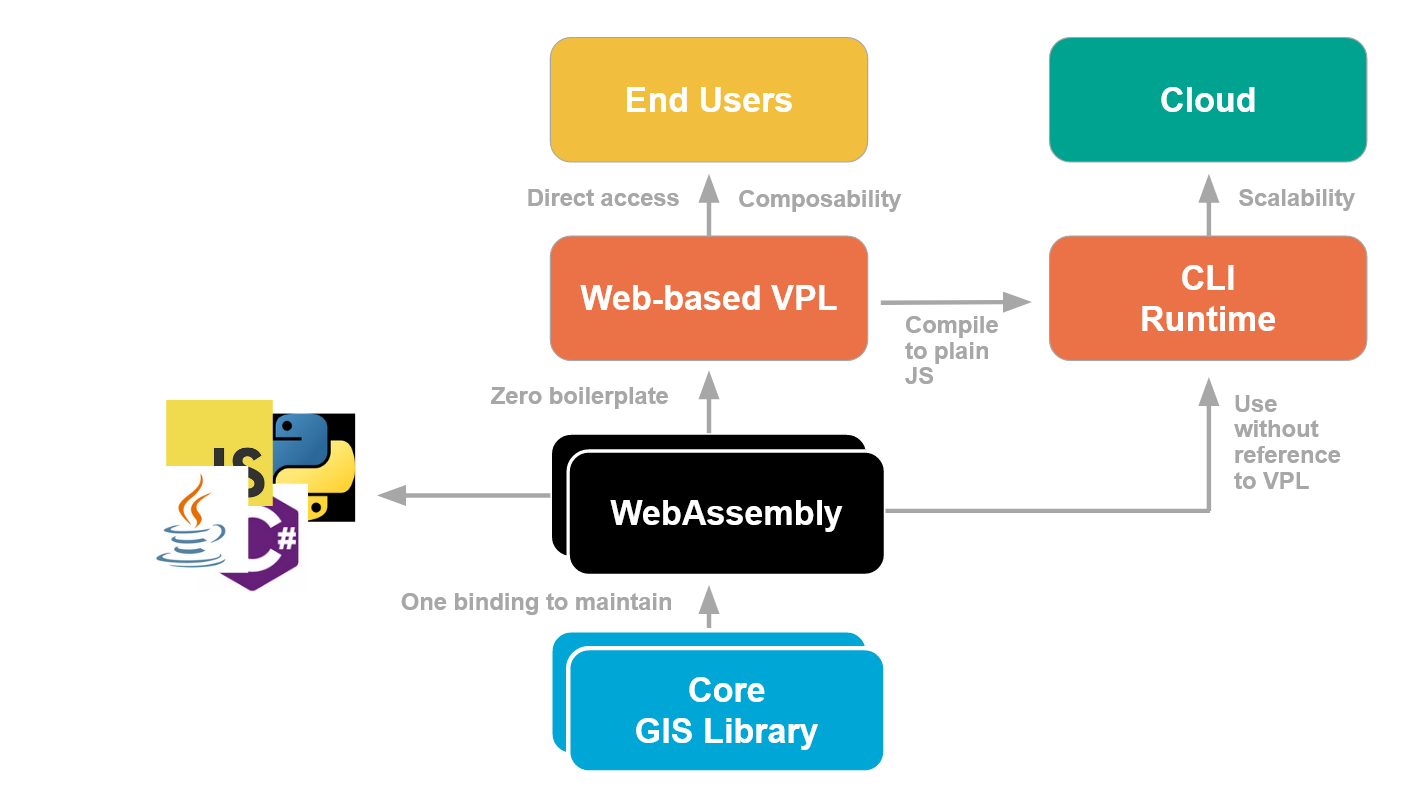
\includegraphics[width=\linewidth]{expanded-proposal.png}
  \end{subfigure}%
  \caption{The methodology expanded beyond the scope of this study, to provide a method for backend, cloud-based execution}
  \label{fig:proposal-extended}
\end{figure}

All in all, to allow for zero-cost abstraction in the future, and allow the \\ zero-boilerplate
concept currently, The plugin system of the proposed method will designed as mentioned above. 

\subsection{Components}

The components mentioned above fit together to propose the following workflow to use a native GIS library in the proposed Web VPL: 
\begin{enumerate}
  \item Write or find a GIS library written in either C++ or Rust. 
  \item Create a second library, in which a subset of this \\ 
  library is flagged and wrapped as 'functions usable on the web'.
  \subitem Optional: Include metadata to add additional functionality to the library
  \item Compile this library with a compatible compiler.
  \item Publish the results of these compilers to a \ac{CDN}. 
  
  \item Within the VPL: Reference the CDN address to the plugin loader. 
  \item The plugin loader now loads and converts the exposed functions, and includes them in the list of VPL components, ready to be used in the VPL. 
\end{enumerate}

For the scope of this system, we will refer to a native GIS library compiled to \\ WebAssembly as a 'plugin', even though these projects are in essence normal JavaScript libraries, and can be used in regular JavaScript projects. 

What follows is an elaboration on the side of the plugin model:

\subsection{Plugin Model}

The plugin model serves three purposes:

\subsubsection{Compilation}

One, it needs to form a bridge between the language in which the GIS library is written, and WebAssembly. 
In other words, the requirements of the WebAssembly compiler compatible with the language in question must be adhered to.
 
The aforementioned WebAssembly interface types proposal is not ready to use for C or C++ based GIS libraries.  
However wrapping WebAssembly using JavaScript types is something C++ does support. 
This can also leverage the infrastructure of JavaScript:
Existing JavaScript tooling, such as \ac{CDN}s, can be utilized for distribution, updates and version control.
Therefore, the WebAssembly binaries will be accompanied by a Javascript wrapper file.

Both the C++ and Rust compilers require functions to be flagged explicitly for compilation. 
Additionally, for a library to be compilable, all dependent libraries must also be able to compile to wasm.
For C++, the Emscripten compiler can be used to compile to WebAssembly \citep*{zakai_emscripten_2011}. 
% A minimum example of what a 'emscripten-ready-library' looks like can be seen in \reffig{fig:minimum-cpp-wasm}.

For Rust, the 'wasm-pack' and 'wasm-bindgen' toolkits enable \ac{wasm} compilation \citep{contributors_wasm-bindgen_2022,contributors_wasm-pack_2022}.
% A minimum example of what this looks like can be seen in \reffig{fig:minimum-rust-wasm}.
% These toolkits do not require incremental compilation steps.
% What is needed, however, is to make sure all dependencies do not use incompatible features, like os file system access. 
% Fortunately, most Rust libraries are written with 'no-std' use-cases in mind, and contain flags to easily exclude these features. 

\subsubsection{Wrapping}

Secondly, in certain situations, some level of function wrapping may still be required. 
Some libraries are written in an imperative style, troubling its conversion to the functional model used by a dataflow VPL (See \reffig{fig:oop-considered-harmful}).
This is why the implementation of this plugin model must take cases like these into account. 
This comes down to wrapping the functionality of the GIS library as pure functions, by making copies of inputs / outputs, or grouping a series of imperative steps.

\begin{figure}
  \centering
  \graphicspath{ {../../assets/images/6/3/} }
  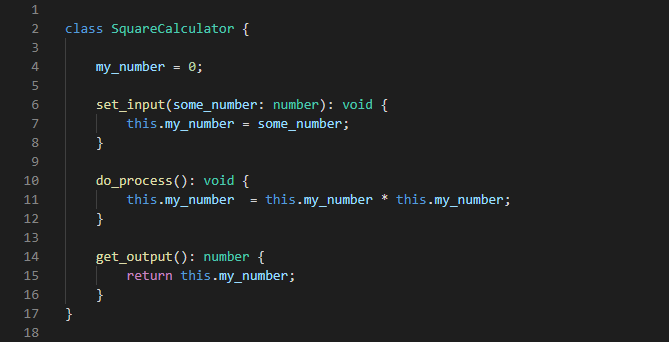
\includegraphics[width=\linewidth]{ugly-oop.png}
  \caption[]{An API which can only be used in an imperative, non-functional manner}
  \label{fig:oop-considered-harmful}
\end{figure}

\subsubsection{Flagging}

Lastly, a plugin model will need to communicate the content of the plugin to the VPL. 
We distinguish between \emph{required} data, and \emph{optional data}.
The central idea for this aspect is to generate this information automatically from the wasm binary and related files.
Only when that is impossible, should the information be manually added within the plugin.

The following information is \emph{required} for the VPL to load a GIS library, and convert it into visual components:

\begin{enumerate}[-]
  \item A list of all functions present in the library, uniquely named.
  \item A list of all custom types (structs / classes) present in the library, also uniquely named.
  \item Per function:  
  \subitem A list of all input parameters, name and type.
  \subitem An output type.
\end{enumerate}

The following information is \emph{optional}, but it would improve the functionality and usability of the library:
\begin{enumerate}[-]
  \item Per function:
  \subitem A custom, human-readable name.
  \subitem A description to explain usage.

  \item Per type:
  \subitem A custom, human-readable name.
  \subitem A description to explain usage.
  \subitem Functions for serializing and deserializing this type (binary, json)  
  \subitem Functions for rendering this type in 2D or 3D.
  \subitem A 'constructor' and 'deconstructor', to convert this type from and to basic types present within the VPL.  
\end{enumerate}

% \begin{figure}
%   \centering
%   \graphicspath{ {../../assets/diagrams/} }
%   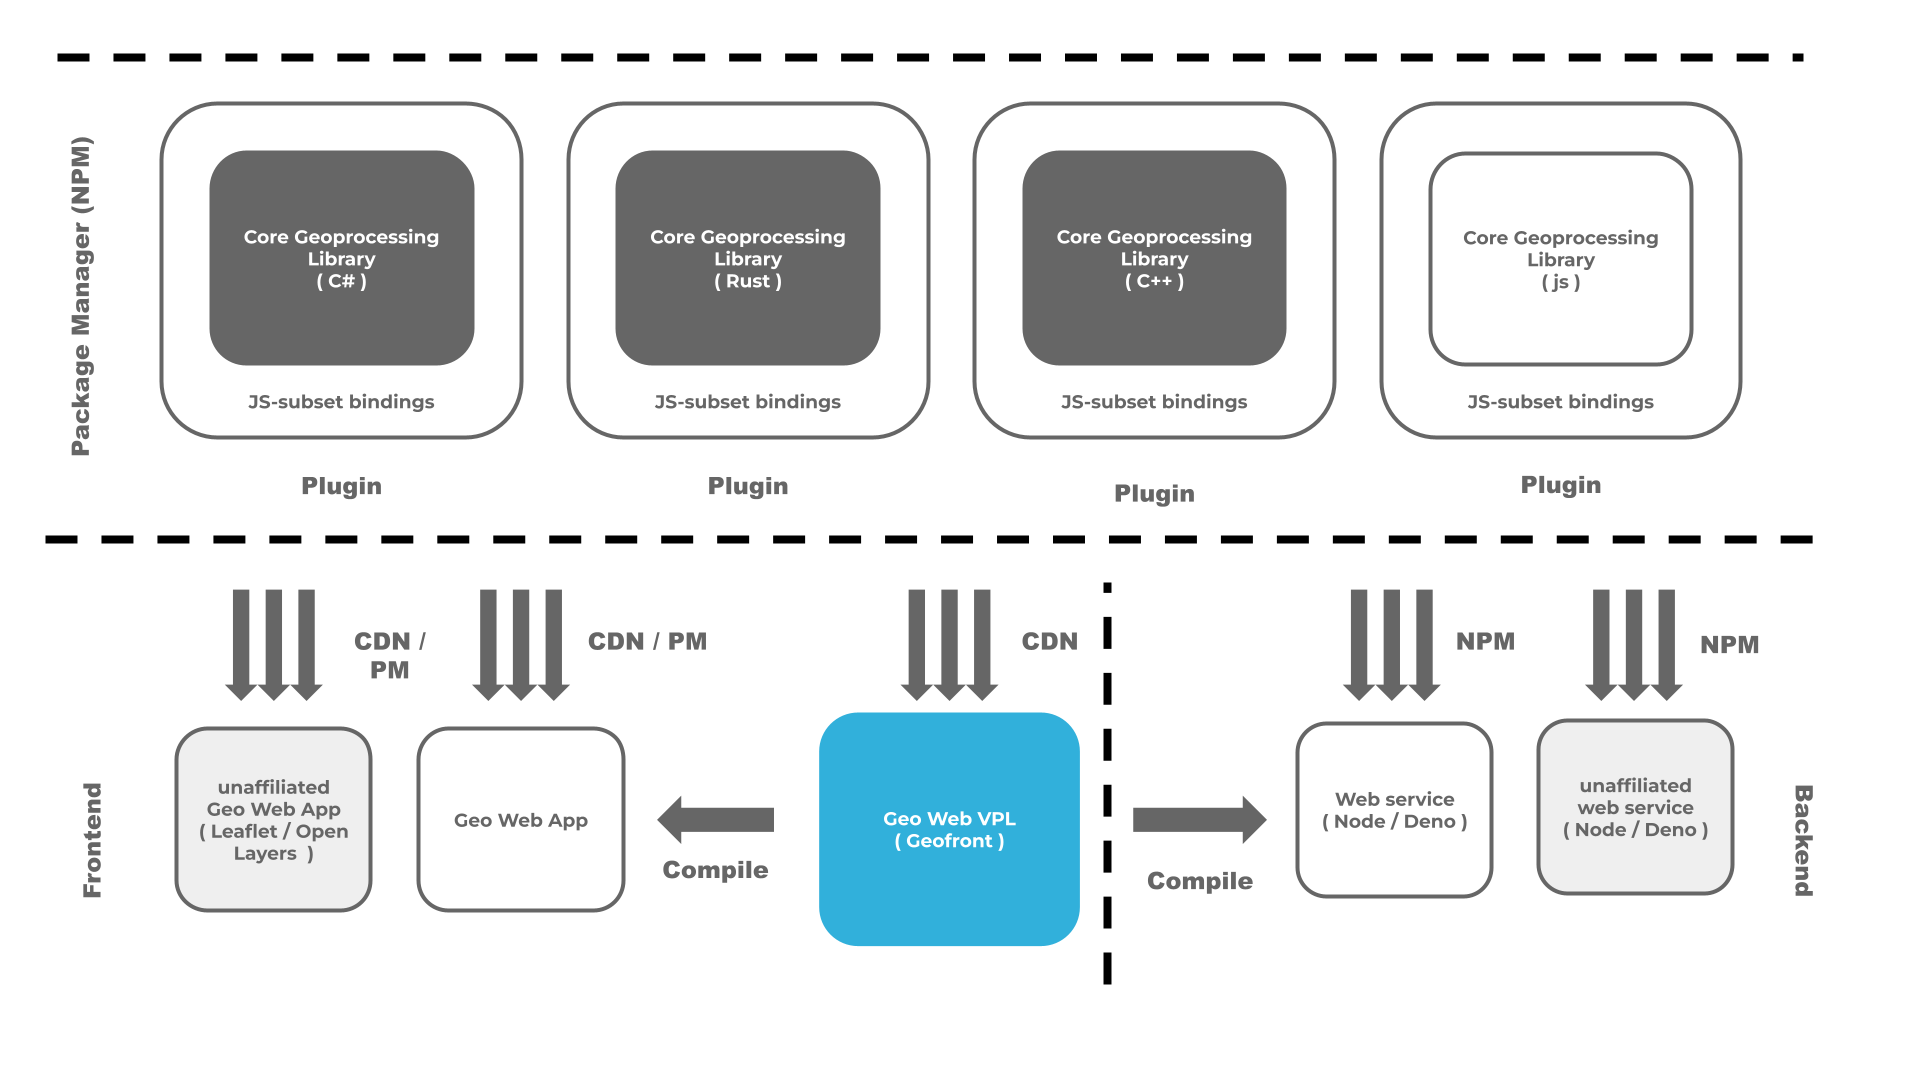
\includegraphics[width=\linewidth]{Model Proposal.png}
%   \caption{TODO: Proposed Plugin model with flagged functions}
%   \label{fig:plugin-model}
% \end{figure}

% \subsection{Plugin Loader}

% \begin{figure}
%   \centering
%   \graphicspath{ {../../assets/diagrams/} }
%   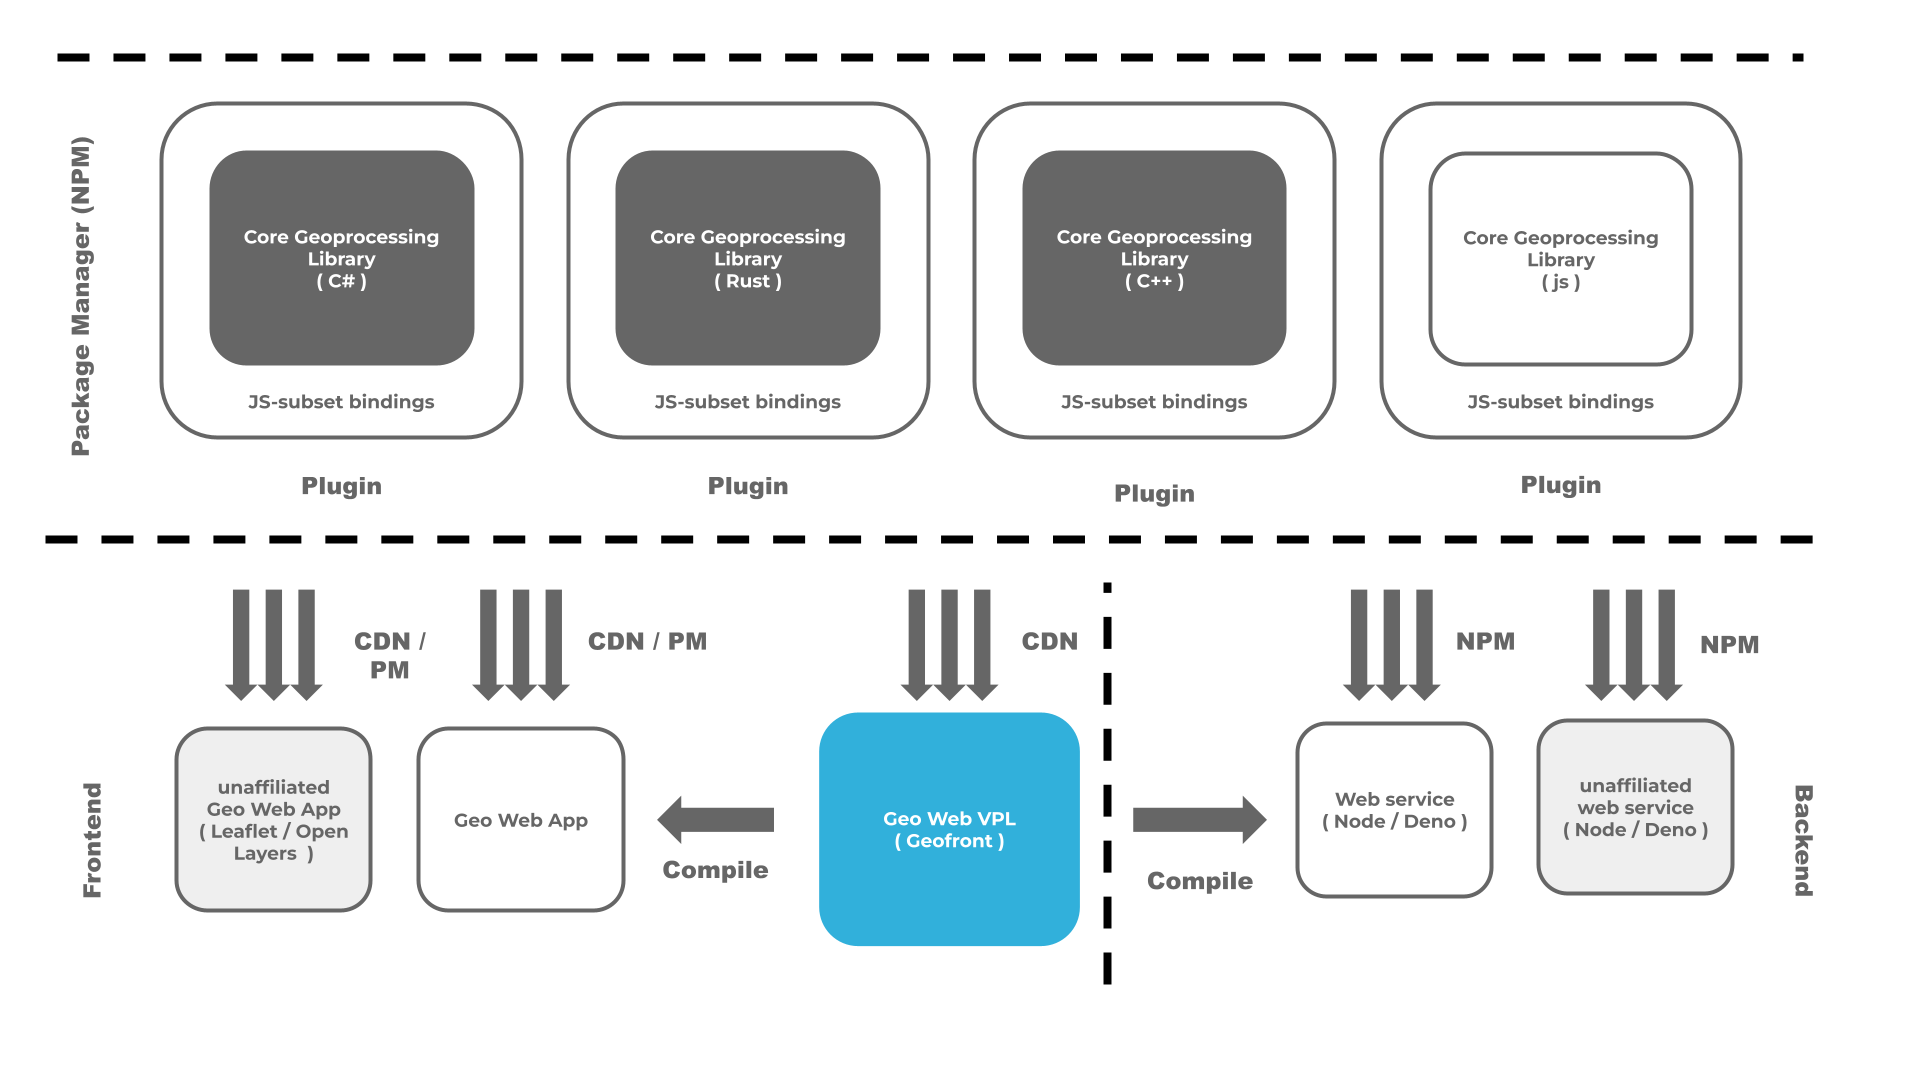
\includegraphics[width=\linewidth]{Model Proposal.png}
%   \caption{TODO: JavaScript \& d.ts headers}
%   \label{fig:plugin-model}
% \end{figure}

On the side of the plugin loader within the VPL, all the compiled, wrapped and flagged information within the plugin needs to be extracted. 
The automated extraction of all \textbf{required} information can be done by utilizing TypeScript Declaration 'd.ts' files. 
A 'd.ts' file can be understood as a 'header' file generated by the TypeScript compiler, exposing the types required by all functions found in a corresponding JavaScript file.
By using the typescript compiler in the VPL, this header file could be loaded and interpreted to find all basic information, including the names, the namespace where to find a functions, and all input and output types.
This extraction of types was required, since these are not present in JavaScript source code, and types are needed in explaining to the end-user how to use a function, and in making the VPL typesafe.

With the extracted information from the "d.ts" file, a corresponding Javascript file can be traversed and loaded as a VPL plugin. 
javascript's nature as a scripting language can be utilized for this:
Firstly, its dynamic nature allowed a library to be loaded and incorporated at runtime without any special alterations. 
Hot-loading libraries in C++ for example, can't usually be done without significantly altering the way a program runs. 
Secondly, JavaScript's prototype-based classes and its support for reflection allows a plugin loader to localize and collect all functions within a library.
And lastly, the "first-class function support" allowed these functions to be referenced and called by the nodes of the VPL Graph. 

Because the VPL will be implemented as a Dataflow-VPL, the loader seeks to extract only (pure) functions. 
However, many libraries also include classes, as these can make an API more clear to use using regular languages. 
The plugin loader will need to support classes by converting them to a series of normal functions. 
Static methods and constructors can be converted directly, and methods are converted into functions with the object as the first argument.

The \textbf{optional} data can be exposed by flagging functions with a standard prefix.
These functions are then loaded by the VPL, but will not be converted into visual components. 
Instead, these functions are programmatically called when the VPL engine or the user requires this optional aspect. 

%%%%%%%%%%%%%%%%%%%%%%%%%%%%%%%%%%%%%%%%%%%%%%%%%%%%%%%%%%%%%%%%%%%%%%%%%%%%%%%
%%%%%%%%%%%%%%%%%%%%%%%%%%%%%%%%%%%%%%%%%%%%%%%%%%%%%%%%%%%%%%%%%%%%%%%%%%%%%%%
%%%%%%%%%%%%%%%%%%%%%%%%%%%%%%%%%%%%%%%%%%%%%%%%%%%%%%%%%%%%%%%%%%%%%%%%%%%%%%%
%%%%%%%%%%%%%%%%%%%%%%%%%%%%%%%%%%%%%%%%%%%%%%%%%%%%%%%%%%%%%%%%%%%%%%%%%%%%%%%
%%%%%%%%%%%%%%%%%%%%%%%%%%%%%%%%%%%%%%%%%%%%%%%%%%%%%%%%%%%%%%%%%%%%%%%%%%%%%%%





\section{Tests}
\label{sec:method:tests}
% The purpose of this final step of the methodology
With both the VPL and the plugin system in place, the final step of the methodology is introduced to gather the results and data needed for properly answering the second, third fourth sub-research questions.

\subsection{Compilation Tests}
\label{sec:method:tests:compilation}

To test the ability of the VPl and the plugin system to host different libraries and different languages, four demo plugins are compiled and loaded within the VPL.  
The Rust language and C++ are tested. 
Per test, the workflow layed out in \refsec{sec:method:plugin-system} is followed. 
Per language, a minimum plugin is first created, assessing if and how well a simple function, method, and class can be exposed to the VPL.
After this demo, a more sizable, existing geocomputation library is compiled.

These tests are meant as a qualitative comparison between compiling a full-scale library written in Rust, to a full library written in C++. 
This way, the tooling and workflow can be compared for a realistic use-case. 
The study is conducted by compiling both libraries using their respective \ac{wasm} toolsets, and noting the differences in workflow, supported features, and the resulting plugins. 

The libraries must be compiled without 'disruption': They must be kept the exact same for normal, native usage. 

\subsubsection{C++ Library: CGAL} 
The library tested for C++ is CGAL, compiled using \m{emscriptem}. 
For one, this library is well established and relevant to geoprocessing as a whole, as multiple other C++ geo-libraries depend on it.
Moreover, it is a sizable and complex project, making it highly likely the problems described by \refsec{sec:background-wasm} are encountered. 
We could choose more simple libraries, but this is not representative of most C++ geoprocessing libraries. 

% \begin{note}
%   HUGO: GDAL-JS ???
%     L takes some time to convert it to a functional model
%     L cannot be used by the plugin system directly, but can be used as a dependency in geofront itself.
%   STARTIN: small s
% \end{note}

\subsubsection{Rust Library: Startin}
The second library tested is the Startin library, written in Rust, compiled using \m{wasm-bindgen}.  
This library is smaller in scope than CGAL. 
Ideally, a library with a size comparable to CGAL should have been chosen, to make for a balanced comparison. 
However, Rust is still a relatively unknown language in the field of GIS, making libraries like these difficult to find. 
Startin was chosen, for the triangulation functionalities it provides makes for a good comparison against CGALs Triangulator. 
It also, just like CGAL, makes use of a high precision kernel, and offers geometric robustness. 

\subsection{Demo applications}

Two demo applications are to be created for the purpose of testing the practical capabilities of the methodology. 
The first demo focusses on the intended use case of 'library publication'. 
We wish to see to what extent a library published using WebAssembly can directly be tested from within the proposed environment. 

The second demo expands upon this first demo, and is intended to examine to what extent such a library can actually be composed as part of a 'real' application. 
In this test, the interaction between this library and the composable \ac{GUI} will be elaborated upon.

% This will be done by using the VPL and plugin loader to create an application. 
% This application, and the process to create it, will then be assessed.

% \subsubsection{Application}

% \begin{note}
% TODO: make a point cloud -> dtm obj tool / isocurves svg / tool
% \end{note}

% \subsubsection{First Experiment}
% The first experiment compares three different methods of bringing the same geocomputation procedure to the web. 
% This way, quantitative, measurable aspects of these methods can be compared. 
% The following three methods are tested:
% \begin{enumerate}[-]
%   \item Write the procedure in normal JavaScript
%   \item Write the procedure in C++, compile to wasm using the \m{emscriptem} toolkit (Source)
%   \item Write the procedure in Rust, compile to wasm using the \m{wasm-bindgen} toolkit (Source)
% \end{enumerate}
% These procedures are all tested within the same web application, using the same data. 
% By taking two different languages, we can distinguish between shortcomings of \ac{wasm} itself, and the \ac{wasm} support of a language.  

% The procedure chosen is a 2D convex hull calculation of a set of sample points. 
% The chosen procedure must be small enough to clearly reason about performance differences, and yet large enough to pose a substantial computational challenge, validating the usage of \ac{wasm}.

% The studies on browser-based geocomputation (\refsec{sec:related-geoweb}) appear to have conducted a similar experiment, by comparing the same procedure written in C++ and JavaScript. 
% However, these studies compared JavaScript against a native, non-web compilation of C++. 
% This experiment also differs in distinguishing between \ac{wasm} itself, and a language's \ac{wasm} support.

% %%%%%%%%%%%%%%%%%%%%%%%%%%%%%%%%%%%%%%%%%%%%%%%%%%%%%%%%%%%%%%%%%%%%%%%%%%%%%%%

% \subsubsection{Second Experiment

\subsection{Feature Comparrison}
\label{sec:method:tests:features}

In this third set of tests, the achieved functionality of the VPL is compared with the functionality of existing VPL methods. 
This comparisons is made on the base of features relevant to the goal of this study:
\begin{itemize}[-]
  \item Does the VPL allow for plugins: Third party 'nodes'?  
  \item In which language must a third party plugin be written?
  \item Can third party nodes use customly defined types, such as a new class or struct?
  \item Can the VPL be run headless, that is to say, without the \ac{GUI}?
  \item Is the VPL accessible as a static web application?
  \item Does the VPL contain GIS-specific nodes by default?
  \item Does the VPL contain \ac{GUI} nodes, so that users can build custom interfaces?
\end{itemize}

\subsection{Usage tests}

% The second set of tests seek the data needed to answer the question of \mySubRQFourTitle: \mySubRQFour.

This final set of tests are meant to analyze the usability of the visual language itself. 
It allows us to understand the advantages and disadvantages of the more granular language design decisions.

For the assessment criteria, the cognitive dimensions framework of \citet{green_usability_1996} will be used. 
The framework is useful for its focus on language features. 
Also, as commented on in \refsec{sec:background-vpl}, the study has acquired a canonical nature among many VPL researchers for its elaborate examination of the "Psychology of Programming".

The framework presents the following 13 dimensions and accompanying descriptions \citep{green_usability_1996}:
\begin{enumerate}
  \item Abstraction gradient: What are the minimum and maximum levels of abstraction? Can fragments be encapsulated? 

  \item Closeness of mapping: What 'programming games' need to be learned? 
  
  \item Consistency: When some of the language has been learnt, how much of the rest can be inferred? 
  
  \item Diffuseness: How many symbols or graphic entities are required to express a meaning? 
  
  \item Error- proneness: Does the design of the notation induce 'careless mistakes'? 
  
  \item Hard mental operations: Are there places where the user needs to resort to fingers or pencilled annotation to keep track of what's happening? 
  
  \item Hidden dependencies: Is every dependency overtly indicated in both directions? Is the indication perceptual or only symbolic? 
  
  \item Premature commitment: Do programmers have to make decisions before they have the information they need? 
  
  \item Progressive evaluation: Can a partially-complete program be executed to obtain feedback on 'How am I doing'? 
  
  \item Role- expressiveness: Can the reader see how each component of a program relates to the whole? 
  
  \item Secondary notation: Can programmers use layout, colour, other cues to convey extra meaning, above and beyond the 'official' semantics of the language? 
  
  \item Viscosity: How much effort is required to perform a single change? 
  
  \item Visibility: Is every part of the code simultaneously visible (assuming a large enough display), or it it at least possible to juxtapose any two parts side-by-side at will? If the code is dispersed, is it at least possible to know in what order to read it?
\end{enumerate}

As stated by the authors; the purpose of this framework is to make the trade-offs chosen by a language's designer explicit. It is not meant as a 'scoring' system \citep{green_usability_1996}.


%%%%%%%%%%%%%%%%%%%%%%%%%%%%%%%%%%%%%%%%%%%%%%%%%%%%%%%%%%%%%%%%%%%%%%%%%%%%%%%
%%%%%%%%%%%%%%%%%%%%%%%%%%%%%%%%%%%%%%%%%%%%%%%%%%%%%%%%%%%%%%%%%%%%%%%%%%%%%%%
%%%%%%%%%%%%%%%%%%%%%%%%%%%%%%%%%%%%%%%%%%%%%%%%%%%%%%%%%%%%%%%%%%%%%%%%%%%%%%%
%%%%%%%%%%%%%%%%%%%%%%%%%%%%%%%%%%%%%%%%%%%%%%%%%%%%%%%%%%%%%%%%%%%%%%%%%%%%%%%
%%%%%%%%%%%%%%%%%%%%%%%%%%%%%%%%%%%%%%%%%%%%%%%%%%%%%%%%%%%%%%%%%%%%%%%%%%%%%%%

%%%%%%%%%%%%%%%%%%%%%%%%%%%%%%%%%%%%%%%%%%%%%%%%%%%%%%%%%%%%%%%%%%%%%%%%%%%%%%%
%%%%%%%%%%%%%%%%%%%%%%%%%%%%%%%%%%%%%%%%%%%%%%%%%%%%%%%%%%%%%%%%%%%%%%%%%%%%%%%
%%%%%%%%%%%%%%%%%%%%%%%%%%%%%%%%%%%%%%%%%%%%%%%%%%%%%%%%%%%%%%%%%%%%%%%%%%%%%%%
%%%%%%%%%%%%%%%%%%%%%%%%%%%%%%%%%%%%%%%%%%%%%%%%%%%%%%%%%%%%%%%%%%%%%%%%%%%%%%%
%%%%%%%%%%%%%%%%%%%%%%%%%%%%%%%%%%%%%%%%%%%%%%%%%%%%%%%%%%%%%%%%%%%%%%%%%%%%%%%


%% OLD STUFF



%%%%%%%%%%%%%%%%%%%%%%%%%%%%%%%%%%%%%%%%%%%%%%%%%%%%%%%%%%%%%%%%%%%%%%%%%%%%%%%

%%%%%%%%%%%%%%%%%%%%%%%%%%%%%%%%%%%%%%%%%%%%%%%%%%%%%%%%%%%%%%%%%%%%%%%%%%%%%%%






% \begin{enumerate}[-]
%   \item Develop a representative use-case application within the prototype \ac{geo-web-vpl}.
%   \item Develop a command line application capable of the very same process.
%   \item Assess both applications according to a series of assessment questions.
% \end{enumerate}

% The execution of this component of the methodology is found in \refsec{sec:analyses:utilization}.

% \subsection{use-case application}
% The application used in both test cases is an "isocurves from DTM" process. 
% But also: we want the iso-curves of a specific location. How to get this data is part of the exercise

% \begin{note}
% [This is subject to change, according to how much I can accomplish ]

% - find the required height data as WFS / WMS
% - determine a boundary
% - load a dtm as a regular png / tiff image
% - specify the parameters, like height delta, smoothness.
% - marching squares
% - post-process curves
% - save as wkt, geojson, or some other well-known vector format

% \end{note}

% Nielsen and Molichs 10 User Interface Design Guidelines
% https://theomandel.com/resources/golden-rules-of-user-interface-design/
% https://www.interaction-design.org/literature/article/user-interface-design-guidelines-10-rules-of-thumb
% (old rules, but still relevant)_
